\documentclass[border=10pt]{standalone}
\usepackage{pgfplots}
\pgfplotsset{compat=1.18}
\begin{document}
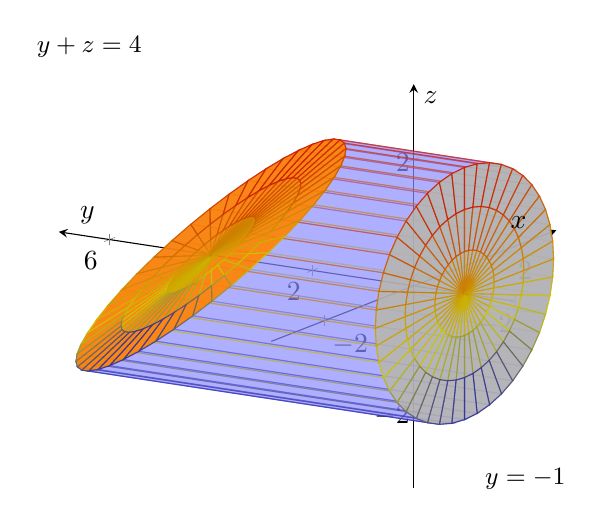
\begin{tikzpicture}
\begin{axis}[
  view={-58}{18},
  axis lines=center,
  xlabel=$x$, ylabel=$y$, zlabel=$z$,
  width=11cm, height=9cm,
  xmin=-3.2, xmax=3.2, ymin=-2, ymax=7, zmin=-3.2, zmax=3.2,
]
% lateral surface, from y=-1 up to y=4-z
\addplot3[surf, color=blue!45, opacity=0.45, domain=0:360, y domain=0:1,
  samples=45, samples y=2]
  ({2*cos(x)}, {-1 + y*(5 - 2*sin(x))}, {2*sin(x)});
% bottom flat cap (disk radius 2) at y=-1
\addplot3[surf, color=gray!60, opacity=0.9, domain=0:360, y domain=0:2,
  samples=45, samples y=4]
  ({y*cos(x)}, {-1}, {y*sin(x)});
% top slanted cap at y=4-z
\addplot3[surf, color=orange, opacity=0.9, domain=0:360, y domain=0:2,
  samples=45, samples y=4]
  ({y*cos(x)}, {4 - y*sin(x)}, {y*sin(x)});
\node at (axis cs:0,-2.2,-2.8) {\small $y=-1$};
\node at (axis cs:0,6.4,3.0) {\small $y+z=4$};
\end{axis}
\end{tikzpicture}
\end{document}
